% Lecture Template for ME3001-001-Tristan Hill - Spring 2017
% 
% Mechanical Engineering Analysis with MATLAB
%
% Roots of Non- Linear Equations - Lecture 3
% MATLAB review

% Document settings
\documentclass[11pt]{article}
\usepackage[margin=1in]{geometry}
\usepackage[pdftex]{graphicx}
\usepackage{multirow}
\usepackage{setspace}
\usepackage{hyperref}
\usepackage{color,soul}
\usepackage{fancyvrb}
\usepackage{framed}
\usepackage{wasysym}
\usepackage{multicol}

\pagestyle{plain}
\setlength\parindent{0pt}
\hypersetup{
    bookmarks=true,         % show bookmarks bar?
    unicode=false,          % non-Latin characters in Acrobat’s bookmarks
    pdftoolbar=true,        % show Acrobat’s toolbar?
    pdfmenubar=true,        % show Acrobat’s menu?
    pdffitwindow=false,     % window fit to page when opened
    pdfstartview={FitH},    % fits the width of the page to the window
    pdftitle={My title},    % title
    pdfauthor={Author},     % author
    pdfsubject={Subject},   % subject of the document
    pdfcreator={Creator},   % creator of the document
    pdfproducer={Producer}, % producer of the document
    pdfkeywords={keyword1} {key2} {key3}, % list of keywords
    pdfnewwindow=true,      % links in new window
    colorlinks=true,       % false: boxed links; true: colored links
    linkcolor=red,          % color of internal links (change box color with linkbordercolor)
    citecolor=green,        % color of links to bibliography
    filecolor=magenta,      % color of file links
    urlcolor=blue           % color of external links
}

% assignment number 
\newcommand{\NUM}{2} 
\newcommand{\VSpaceSize}{2mm} 
\newcommand{\HSpaceSize}{2mm} 

\definecolor{mygray}{rgb}{.6, .6, .6}

\setulcolor{red} 
\setstcolor{green} 
\sethlcolor{mygray} 

\begin{document}

\textbf{ \LARGE ME 3001 Lecture, Roots of Non-Linear Equations} \\\\
\textbf{ \LARGE A Brief Refresher in MATLAB} \\

\begin{itemize}

	\item  \textbf{\LARGE What is it?}
		\LARGE
		\begin{itemize}
			\item High Level programming language
				\begin{itemize}
					\item language written in C++
					\item Interactive Development Environment written in JAVA 
					\item Windows, Mac, and Linux compatable
				\end{itemize}
			\item {\it MAT}rix {\it LAB}oratory
			\item {\it Technical Computing Language} - Mathworks
		\end{itemize}	

	\item \textbf{\LARGE Why use it?}
		\begin{itemize}
			\item A powerful tool for engineers, scientists, and students
				\begin{itemize}	
					\item  optimized for floating point arithmetic and linear algebra
					\item extensive library of mathematical functions and operations 
					\item specialized functions and operations
						\begin{itemize}
							\begin{multicols}{2}
							\item Aerospace
							\item Robotics
							\item Communications
							\item Image/Signal Processing 
							\item Embedded Systems and Controls
							\end{multicols}
						\end{itemize}
					\item ability to use {\it symbolic programming }	
				\end{itemize}
			\item Ease of Access and Community
				\begin{itemize}
					\item {\it Plug and Play}, it works out of the box
					\item requires little or no programming experience to begin
					\item online community for sharing code,  {\it MATLAB Central}
				\end{itemize}
		\end{itemize}

\item \textbf{\LARGE Why Not?}
\newpage

\item \textbf{\LARGE Review of some basic MATLAB}

	\begin{itemize}

		\item \textbf{ \LARGE Useful Commands( type in Command Window)}\\

		
			\scalebox{1.5}{{\fontfamily{qcr}\selectfont  \hspace{5mm} >>  clear variables}} \\\\
			\scalebox{1.5}{{\fontfamily{qcr}\selectfont  \hspace{5mm} >>  clc}} \\\\
			\scalebox{1.5}{{\fontfamily{qcr}\selectfont  \hspace{5mm} >>  close all}} \\\\
			\scalebox{1.5}{{\fontfamily{qcr}\selectfont  \hspace{5mm} >>  }} \\\\



		\item \textbf{ \LARGE Built-In MATLAB functions}\\
	
		
			\begin{itemize}
				\item \textbf{\Large Typical Mathematics Functions} \\	
					\begin{itemize}
						\item \scalebox{1.5}{{\fontfamily{qcr}\selectfont  \hspace{5mm} sqrt()}} \\
						\item \scalebox{1.5}{{\fontfamily{qcr}\selectfont  \hspace{5mm} exp()}} \\
						\item \scalebox{1.5}{{\fontfamily{qcr}\selectfont  \hspace{5mm} log()}} \\
						\item \scalebox{1.5}{{\fontfamily{qcr}\selectfont  \hspace{5mm} log2()}} \\
						\item \scalebox{1.5}{{\fontfamily{qcr}\selectfont  \hspace{5mm} log10()}} \\
					\end{itemize}	
				\newpage
				\item \textbf{\Large Other Useful Functions} \\	
					\begin{itemize}
						\item \scalebox{1.5}{{\fontfamily{qcr}\selectfont  \hspace{5mm} round()}} \\
						\item \scalebox{1.5}{{\fontfamily{qcr}\selectfont  \hspace{5mm} floor()}} \\
						\item \scalebox{1.5}{{\fontfamily{qcr}\selectfont  \hspace{5mm} int8()}} \\
						\item \scalebox{1.5}{{\fontfamily{qcr}\selectfont  \hspace{5mm} sign()}} \\
						\item \scalebox{1.5}{{\fontfamily{qcr}\selectfont  \hspace{5mm} mod()}} \\
						\item \scalebox{1.5}{{\fontfamily{qcr}\selectfont  \hspace{5mm} rem()}} \\
						\item \scalebox{1.5}{{\fontfamily{qcr}\selectfont  \hspace{5mm} fzero()}} \\
					\end{itemize}	

				\item \textbf{\Large The Built in Help }\\	
					\begin{itemize}
						\item \scalebox{1.5}{{\fontfamily{qcr}\selectfont  \hspace{5mm} >> help fzero()}} \\
						\item \LARGE{use the help to get information about the built in functions } \\
						\item \LARGE{the full documentation is also available online } \\\\
						
					\end{itemize}	
				\newpage
			\end{itemize}

	\newpage
	\item \textbf{ \LARGE Constants} \\

		 \LARGE{Several useful constants are built into MATLAB.} \\

				\begin{itemize}
					
					\item \scalebox{1.5}{{\fontfamily{qcr}\selectfont  \hspace{5mm} pi}} \\
					\item \scalebox{1.5}{{\fontfamily{qcr}\selectfont  \hspace{5mm} i}} \\
					\item \scalebox{1.5}{{\fontfamily{qcr}\selectfont  \hspace{5mm} j}} \\
					\item \scalebox{1.5}{{\fontfamily{qcr}\selectfont  \hspace{5mm} inf}} \\
					\item \scalebox{1.5}{{\fontfamily{qcr}\selectfont  \hspace{5mm} NaN}} \\\\

				\end{itemize}


	

	\item \textbf{ \LARGE Random Numbers} \\
		
			 \LARGE{Sometime it is useful generate random data in MATLAB.} \\

				\begin{itemize}
					
					\item \scalebox{1.5}{{\fontfamily{qcr}\selectfont  \hspace{5mm} rand()}} \\
					\item \scalebox{1.5}{{\fontfamily{qcr}\selectfont  \hspace{5mm} randi()}} \\\\\\
		
				\end{itemize}

	\newpage
	\item \textbf{ \LARGE User Defined Functions}\\

				\begin{itemize}

				\item  \LARGE{We often write our own functions in MATLAB. To do this we must define the function in the function file.} \\ \vspace{50mm}

				\item  \LARGE{When we use a function we {\it call} the function.} \\ \vspace{50mm}
					
				\item  \LARGE{we can refer to a function with {\it handle operator}} \\ \vspace{50mm}
				
		
				\end{itemize}

	\end{itemize}

\newpage

\item \textbf{\LARGE A Mechanical Design Problem}\\\\	
		
		As an engineer you are asked to design a structure. The geometery of these structures is simple but certain properties are critical. Also you want to spend as little as possible on materials.
		
	
		
		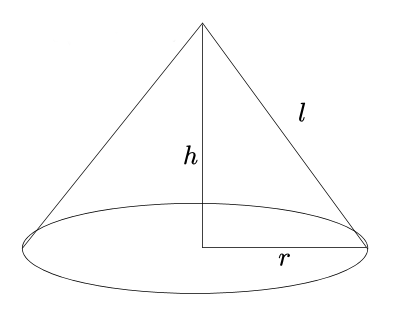
\includegraphics[scale=.5]{lecture3_fig1.png}\\
		
		  \scalebox{1.2}{surface area, $s=\pi r l = \pi r \sqrt{h^2+r^2}$} \\\\

		

		

			
		The first structure you are required to design is a cone with a surface area of exactly $100 m^2$ to a tolerance of 0.1 $m^2$ and a height of exactly $1 m$. Your goal is to find the radius in meters.\\

Write a program the uses the {\it Newton -Raphson} method to solve the problem. Verify and compare your answer with the {\it fzero} function. \vspace{20mm}
				
			
		 
			



\newpage 

	\item \textbf{ \LARGE REMINDER - Homework 1 is due Friday } \\
	 
	\item \textbf{ \LARGE REMINDER - MATLAB script from today's lecture will be posted on ilearn. } \\

\end{itemize}


	

\end{document}



